\chapter{Fundamentals}
\label{ch:Fundamentals}
This chapter provides fundamental information about the techniques and notation used in the approach. As introduced in Chapter \ref{ch:CoCoME}, the Case Study's system specification is given in terms of detailed use cases. However, the proposed approach uses business processes as input. The following sections introduce a well known and established use case notation technique, a standardized notation to capture business processes and a structured approach to transform use case sets as business processes. 


\section{Use Cases}
\label{sec:Fundamentals:UC}
Use Cases are a widely adopted technique to document software system requirements. Generally, they describe the interaction between actors (usually system users) and the software system itself. In this thesis, use cases need to be provided as semi-structured tables (following the notation presented by Cockburn et al. \cite{Cockburn}). \\ An example is given in Table \ref{tab:exampleUseCase}: Each use case has a unique identifier and a short description, followed by necessary preconditions and a trigger that causes the execution. The standard process is the main part and describes the success steps of the Use Case. Extensions provide additional information like alternatives or exceptional processes that occur in case of an unsuccessful step. 




\begin{table}[!h]
	\centering
	\begin{tabularx}{\textwidth}{|l||X|}
		\hline
	    UC 5 & Show Stock Reports \\ 
	    \hline
	    Brief Description &  The opportunity to generate stock-related reports is provided
	    by the Trading System. \\
	    \hline
	    Precondition & The reporting GUI at the Store Client has been started. \\
	    \hline
	    Trigger & The Store Manager wants to see statistics about his store. \\
	    \hline
	    Postcondition & The report for the Store has been generated and is displayed on
	    the reporting GUI. \\
	    \hline 
	    Standard Process &
	       
	            1. The Store Manager enters the store identifier and presses the button Create
	                     Report.  \\
	           & 2. A report including all available stock items in the store is displayed. \\  
        \hline
        Extensions & (none) \\ \hline
	   
		
	\end{tabularx}
	\caption{Example Use Case in Tabular Form, Source: \cite{CoCoMEOld}}
	\label{tab:exampleUseCase}
	
\end{table}

\noindent
The usage of Use Cases as input for the approach has a remarkable benefit: Besides being a widely adopted technique to specify system requirements, the textual use case notation is understandable without further technical knowledge. Neither previous knowledge in specific graphic notations like UML, nor the capability to create a complex domain model is necessary. Consequently, all sort of stakeholders (non-technical and technically experienced) are capable to provide the necessary information in terms of use cases. 





\section{Business Process and Model Notation}
\label{sec:Fundamentals:BPMN}
The Business Process and Model Notation (BPMN) is a graph oriented language to describe business processes. Originally, BPMN was designed to describe activities and their control flow dependencies only \cite{VisualizeBPMN}. Since the introduction of BPMN 2.0, it is possible to model the data needs and the data results of activities \cite{OMG}. Consequently, BPMN is capable to express the control flow and data flow of business processes \cite{DataFlowErrorBPMN}. In the remainder, we use BPMN instead of BPMN 2.0 for the sake of convenience. \\
BPMN is easy-to-use, powerful and widely adopted in academia and industry. Hence, BPMN is a suitable approach to extract the implicitly given data flow and control flow in the use case description. Sec. \ref{sec:Fundamentals:TransformUCtoBPMN} introduces a formal approach to generate BPMN processes from use case sets. Next, the BPMN 2.0 process definition is shortly introduced:


\begin{figure}[h!]
	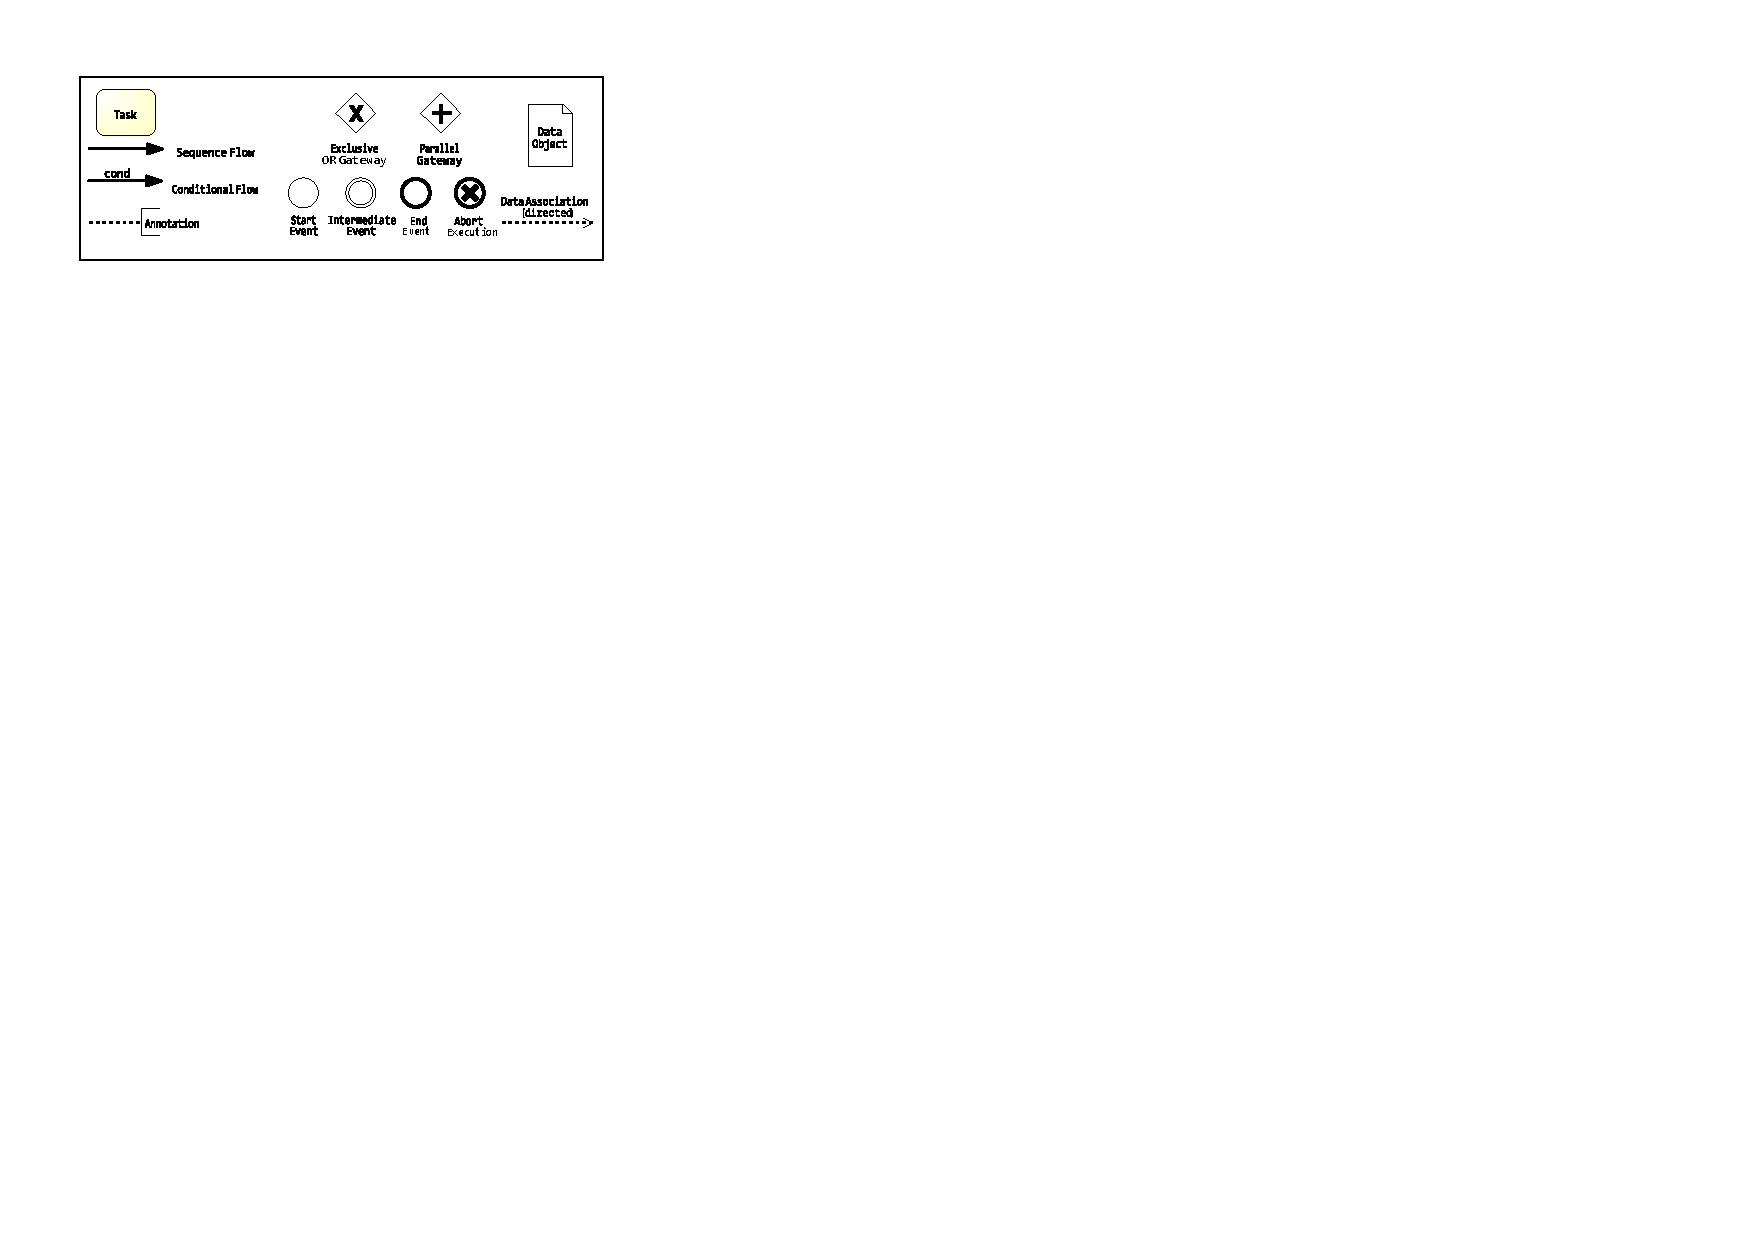
\includegraphics[width=\textwidth, trim={1cm 16.5cm 19.2cm 1cm}]{img/Overview.pdf}
	\caption{BPMN Notation (Subset)}
	\label{fig:BPMNSubset}
\end{figure}





\section{Transform Use Case Sets in BPMN Processes}
\label{sec:Fundamentals:TransformUCtoBPMN}

